% The pre-analysis plan as a PDF. The text is comparison/survey/PRE-ANALYSIS-PLAN.md, converted by
% build.sh; edit the markdown, not plan-body.tex.
\documentclass[11pt]{article}
\usepackage[margin=1in]{geometry}
\usepackage{amsmath,amssymb,booktabs,graphicx,tabularx,float,longtable,array,calc}
\usepackage[T1]{fontenc}
\usepackage[utf8]{inputenc}
\usepackage{lmodern}
\usepackage{textcomp}
% Appendix A quotes the treatment form's minus sign (U+2212) as the form shows it
\DeclareUnicodeCharacter{2212}{\textminus}
\usepackage{pdfpages}
\usepackage[hidelinks]{hyperref}
\setlength{\parskip}{4pt}
\setlength{\parindent}{0pt}
\providecommand{\tightlist}{\setlength{\itemsep}{0pt}\setlength{\parskip}{0pt}}
\providecommand{\pandocbounded}[1]{#1}
\setcounter{secnumdepth}{0}
\sloppy
\makeatletter\def\verbatim@font{\small\ttfamily}\makeatother

\title{Pre-analysis plan for a study of salience of study information and credibility assessment of key assumptions and inputs}
\author{Fernando Hoces de la Guardia}
\date{19 October 2026}

\begin{document}
\maketitle
\textbf{A note on this document.} This pre-analysis plan was drafted with the assistance of Claude
Code. It is unclear whether the survey will draw any responses at all. The plan was written for
the optimistic case, in which enough people respond for a study to be conducted with the data. It
was written now so that the analysis is fixed before any response is seen. \textbf{At this point, it is the opinion of the
author that no human should spend much time reading this pre-analysis plan. It is only intended
as a record.}

Status: the version registered on the AEA RCT Registry (the American Economic Association's
registry of randomized controlled trials, trial 19997) on 2026-10-19, before the forms open. The structure follows the minimal elements of a clear hypothesis: population,
interventions, arms, outcomes, hypotheses (contrasts, tests, alternative, estimation, standard
errors), and heterogeneity stated separately and in full.

\section{1. Question}\label{question}

Proposition 40 is a California ballot measure. It would tax Californians worth \$1 billion or more
once, at 5\% of their net worth. Two academic studies estimate what the tax is worth to the state:
Boll, Saez and Zucman (the BSZ analysis) and Jaros and Rauh (the JR analysis). One finds that the
tax raises money for the state and the other that it loses money. This project is an Open Policy
Analysis (OPA) of the two. Its website puts both estimates on one measure and shows, on a page
called the comparison explorer, which inputs explain the gap between them. The project's survey
asks respondents which of two proposed values of each disputed input (an input on which the two
analyses use different values) they find more credible. The comparison explorer shows the same
inputs, which study uses which value, and what each value does to the estimate. Most respondents
will have seen that comparison on the site before they open the survey. This study asks whether
the answers change when the comparison is restated at the moment respondents choose the input
values, with each value labelled by its study.

\section{2. Population and sample}\label{population-and-sample}

\begin{itemize}
\tightlist
\item
  \textbf{Population.} Everyone who submits one of the four open forms (section 4.3) during the
  collection window (section 9), whether they reached the form through a project survey link or
  through a form address that someone forwarded (section 8). No one is screened out. Self-described experts and
  respondents without prior exposure are subgroups (section 6), not the sample.
\item
  \textbf{Unit of randomization.} The respondent, drawn at the click on a survey link (section 4.2).
\item
  \textbf{Unit of analysis.} One submitted response.
\item
  \textbf{Sample size.} The sample size is not controlled. It is whoever responds in the window. The number of
  responses depends on whether the launch of the OPA gains traction on social media, and it is
  likely that there will be none or very few. A reasonable range is 0 to 200. The staged rule of section 7 decides which analyses run once the realized number
  is known, and section 7 gives the detectable effects for a range of sizes.
\end{itemize}

\section{3. Interventions}\label{interventions}

There are two manipulations. Both are delivered only in the treatment forms. Nothing is delivered
to the control group, which makes it a pure control.

\begin{itemize}
\tightlist
\item
  \textbf{I1, the comparison page.} This is one page, titled ``How the two estimates differ'', shown after
  the opening questions and before the input questions. It opens with ``Two academic studies'' and gives each
  study on its own bullet with its month and its estimate (Boll, Saez and Zucman, the BSZ analysis, and Jaros and
  Rauh, the JR analysis). Neither bullet names a venue. Both are working papers of the National
  Bureau of Economic Research (NBER). Naming a venue for one study only would signal that it is
  the more reputable one, and that signal would become part of the treatment. It then gives the
  gap between the two estimates and names the common measure on which the explorer puts both.
  Next it splits the gap into the four terms of the comparison explorer's equation (a sum, one
  term per group of inputs, that adds up to the gap), largest first. Each term has a bar, its amount in billions and its share of the gap, and, for
  the first three, the values each study uses. A sentence names the two largest terms and their
  combined share. A two-sentence note says why the lost income tax is one term (explained after the table below) and that
  each amount depends on the order in which the inputs are changed. The full text is in Appendix A.
\item
  \textbf{I2, the study labels.} In the input questions, each choice is labelled with its study (``BSZ:''
  or ``JR:'') instead of ``A.'' or ``B.''. The choice text and order are otherwise unchanged.
\end{itemize}

The four terms, as generated at the launch commit (section 9), follow.\footnote{Each amount is the sum of the explorer's walk steps in that term
  (\texttt{comparison/export/r/dial\_path.csv}). The walk moves the inputs one after another from the BSZ
  values to the JR values. The values come from \texttt{comparison/export/r/inputs.csv}.
  \texttt{comparison/survey/mock\_forms.py} and \texttt{gas\_build.py} generate the page from those files, so no
  number is typed. They also check that every walk step belongs to one term and that the terms
  add up to the gap.} The gap is \$145.8 billion.

{\def\LTcaptype{none} % do not increment counter
\begin{longtable}[]{@{}
  >{\raggedright\arraybackslash}p{(\linewidth - 4\tabcolsep) * \real{0.6000}}
  >{\raggedright\arraybackslash}p{(\linewidth - 4\tabcolsep) * \real{0.1714}}
  >{\raggedright\arraybackslash}p{(\linewidth - 4\tabcolsep) * \real{0.2286}}@{}}
\toprule\noalign{}
\begin{minipage}[b]{\linewidth}\raggedright
Term on the page
\end{minipage} & \begin{minipage}[b]{\linewidth}\raggedright
Amount
\end{minipage} & \begin{minipage}[b]{\linewidth}\raggedright
Share of the gap
\end{minipage} \\
\midrule\noalign{}
\endhead
\bottomrule\noalign{}
\endlastfoot
The income tax lost when billionaires leave: the share lost, how long it is counted, and billionaires' yearly income tax, together & -\$81.3 billion & 56\% \\
Discounting the revenue for court risk & -\$39.4 billion & 27\% \\
Billionaires who moved out in time & -\$29.9 billion & 21\% \\
Other inputs together: the wealth on the list, avoidance, and three smaller inputs & +\$4.9 billion & offsets 3\% \\
\end{longtable}
}

The shares add to 101\% because of rounding. A negative amount means that the term lowers the
estimate as the inputs move from the BSZ values to the JR values, and a positive amount that it
raises it. The page prints the first three amounts without a sign.

The page does not give one amount per survey question. The lost income tax is a product of the
share lost, how long it is counted and the yearly amount. A split among those three factors would
depend on the order in which they are changed, so it would misstate what any one of them does. The
page shows them as one term and says why. As a result, the terms do not match the survey questions
one to one. The first term covers three whole questions: the share lost, how long it is counted,
and the yearly income tax. The question on billionaires who moved out in time spans two terms.
The JR value (seven named moves) is the third term. The BSZ value (an allowance for unnamed
movers, which is half of the BSZ analysis's allowance for avoidance) sits in the fourth term,
together with the rest of that allowance. The two optional questions, on
avoidance and on the wealth the tax applies to, also sit inside the fourth term. Only the court question matches one
term. The small difference in
discount rates is inside the first term and is not named, since the question on how long the lost income tax is counted (the horizon question, section
4.4) no longer asks about it.

\section{4. Arms and assignment}\label{arms-and-assignment}

\subsection{4.1 Arms}\label{arms}

{\def\LTcaptype{none} % do not increment counter
\begin{longtable}[]{@{}lll@{}}
\toprule\noalign{}
Arm & I1 & I2 \\
\midrule\noalign{}
\endhead
\bottomrule\noalign{}
\endlastfoot
Control (T = 0) & no & no \\
Treatment (T = 1) & yes & yes \\
\end{longtable}
}

I1 and I2 are delivered together. The design measures their joint effect and cannot separate them.

\subsection{4.2 Assignment}\label{assignment}

Google Forms cannot randomize inside a form, so the draw happens at the click. Each survey link
opens its entry point's control form or treatment form with probability 1/2, drawn in the browser (\texttt{Math.random()\ \textless{}\ 0.5}). The respondent sees nothing of either form before the draw. Draws are independent. Each entry point is a stratum: a group within which the draw is made, and which the analysis accounts for with its own indicator (section 6.1).

\subsection{4.3 Entry points and forms}\label{entry-points-and-forms}

There are four forms: one control form and one treatment form for each of two entry points. The form a response lands in records its entry point and its arm. Respondents see neither label. Appendix B reproduces the control and treatment forms.

{\def\LTcaptype{none} % do not increment counter
\begin{longtable}[]{@{}
  >{\raggedright\arraybackslash}p{(\linewidth - 6\tabcolsep) * \real{0.1667}}
  >{\raggedright\arraybackslash}p{(\linewidth - 6\tabcolsep) * \real{0.5000}}
  >{\raggedright\arraybackslash}p{(\linewidth - 6\tabcolsep) * \real{0.1667}}
  >{\raggedright\arraybackslash}p{(\linewidth - 6\tabcolsep) * \real{0.1667}}@{}}
\toprule\noalign{}
\begin{minipage}[b]{\linewidth}\raggedright
Entry point
\end{minipage} & \begin{minipage}[b]{\linewidth}\raggedright
Who arrives there
\end{minipage} & \begin{minipage}[b]{\linewidth}\raggedright
Control
\end{minipage} & \begin{minipage}[b]{\linewidth}\raggedright
Treatment
\end{minipage} \\
\midrule\noalign{}
\endhead
\bottomrule\noalign{}
\endlastfoot
\texttt{explorer} & the survey button lower on the explorer page, and the overview page's two survey buttons & form 3 & form 4 \\
\texttt{share} & the share link (\texttt{comparison/site/survey/}): copied from the site, sent by email, or opened from the public posts through tinyurl.com/prop40-survey & form 5 & form 6 \\
\end{longtable}
}

Forms 1 and 2 belonged to a third entry point, \texttt{landing}: a panel shown to every visitor of the
explorer before the results, inviting them to take the survey first. The panel was removed on
2026-10-17, before launch, because it stood between visitors and the explorer and could deter
them from using it. Forms 1 and 2 were built but are never opened.

The OPA pages point readers to the comparison explorer several times, and the explorer shows the
two competing estimates side by side. Every respondent who arrives through the \texttt{explorer} entry
point has therefore seen the comparison before opening the survey. The \texttt{share} link opens a form
directly, so its respondents are a mix: some have seen the estimates and some have not. For this
reason the experiment mainly tests salience, that is, whether bringing that information back to
mind at the moment respondents choose the input values changes the answers, and not the effect of
a first exposure to it.

The \texttt{share} stratum also holds some visitors of the explorer and the overview. A survey button
opened without a click event, through the context menu, a long press or a drag, goes to the share
page, which draws and records in the \texttt{share} stratum (section 8). These visitors have seen the
comparison. Their presence shrinks the difference that H2 looks for and does not touch H1.

\subsection{4.4 Page order (all forms)}\label{page-order-all-forms}

\begin{enumerate}
\def\labelenumi{\arabic{enumi}.}
\item
  The title (``What are the actual quantities? Proposition 40, input by input'') and the
  description, then two pre-treatment questions and the optional email:

  \begin{itemize}
  \tightlist
  \item
    ``Do you consider yourself an expert in tax or fiscal policy?'' (Yes / Somewhat / No; moved here
    from the end of the current survey, the version 1 forms that have been open since before the
    experiment)
  \item
    ``Before opening this survey, had you looked at news sources, web pages or academic studies
    discussing estimates of Proposition 40, the Billionaire Wealth Tax Proposal in California?''
    (Yes / No / Not sure; new)
  \item
    ``Your email (optional)'' (moved here from the closing page on 2026-10-18, so it is asked before
    treatment; nothing is verified)
  \end{itemize}
\item
  I1 (treatment forms only).
\item
  The page ``The inputs'' (``For each input, pick the value you find more credible.''): the five
  required input questions, in three groups under plain section headings, in the order
  of the treatment page's first three terms (\texttt{GROUPS}, \texttt{regroup()} and \texttt{split\_bundle()} in
  \texttt{mock\_forms.py}):

  \begin{itemize}
  \tightlist
  \item
    ``1. The income tax lost when billionaires leave'': ``The share of billionaires' income tax lost
    when people leave: which is more credible?'', then how long the lost income tax is counted,
    then billionaires' yearly income tax. The three are ordered by each input's effect on the
    estimate, averaged over every order in which the explorer's dials (the controls that switch
    each input between its two values) can be turned, largest first.
  \item
    ``2. Discounting the revenue for court risk'': the court question.
  \item
    ``3. Billionaires who moved out in time'': ``Billionaires who moved out of California before
    the 1 January 2026 residency date: which is more credible?'' It spans two of the page's terms
    (section 3).
  \end{itemize}

  Each required question is followed by a free-text box, ``Why? (optional)''. These boxes carry the
  reasons that section 5.3 reports alongside S1.

  Then comes the opt-in to the five smaller inputs, a required question with the choices ``Yes,
  show me the five'' and ``No, skip them''. Their page (``Five smaller inputs (optional)'') follows it
  and asks about wealth that escapes the tax through avoidance and evasion, the wealth the tax
  applies to, non-citizen residents, the real-estate deduction, and the extra income tax from
  assets sold to pay the tax. One ``Why? (optional)'' box closes the optional page.

  The current survey bundles departures, avoidance and the share lost into one question. In all
  the forms that question becomes three: the share lost and moved out in time (both required), and
  avoidance (optional). The two values offered in each of the three then concern one and the same
  input. The wealth question moves
  from the required questions to the optional page. I2 applies to all ten input questions in the
  treatment forms.
\item
  The closing page, ``Anything else (optional)'': missing inputs and support for
  Proposition 40. Every question on it is optional.
\end{enumerate}

The question order and the three headings are the same in both arms, so they are not part of the
treatment. They differ from the current survey's order. All the forms use one fixed choice order
within each question, that of the current survey (version 1). In the first pretest (section 9) the
second-listed value won the share-lost question (21 to 9) and the court question (18 to 4) in the
control forms, so its language-model respondents showed no sign of favouring the first-listed
value. That says little about people. Because the order is the same in both arms, an order effect
cannot bias H1. It can shift the level of each question's answers in S3. The horizon question drops the
discount rate (author, 2026-10-16): ``How long the lost income tax is counted: which is more
credible?'', with the choices ``For ever: billionaires who leave are assumed not to return.'' and ``5
years, about the payment period, treating the departures as temporary.'' (``departures'' replaced
``responses'' on 2026-10-17, because no respondent had been given a meaning for ``responses''). The current survey's
``Which field best describes your work?'' is dropped (author, 2026-10-16).

\textbf{Wording of the values (revised 2026-10-17, after the first pretest, and approved by the author
the same day).} In every input question the two values are the same kind of claim. Each gives a
reason, or neither does. Neither value argues against the other. The texts are generated by
\texttt{mock\_forms.py} (\texttt{SHARE}, \texttt{DEPARTED}, \texttt{AVOID}, \texttt{INCOME}, \texttt{COURT}, \texttt{WEALTH}, \texttt{NONCIT}, \texttt{REAL},
\texttt{ASSET}), with every number read from the exports. What changed, and why:

\begin{itemize}
\tightlist
\item
  The share lost now states both values on the same base, ``of all the income tax that
  billionaires pay'' (\texttt{comparison/DISPUTES.md}, row 6): 45\%, more than the 29\% of wealth reported
  to have left, against 5\%, the same as the 5\% of wealth assumed to leave. Each comes with its
  analysis's own reason. The old pair (``45\% of
  all billionaires' income tax, whoever leaves'' against ``5\%, only the income tax of those who
  leave'') was read in three ways in the first pretest: as a count of leavers, as shares of two different
  bases, and as losing the tax of those who stay. A respondent who accepts one analysis's count
  of the wealth that left but the other analysis's rule for which income tax is lost can now
  answer.
\item
  The court question now asks whether to bring a court-risk discount into the estimate at all.
  Its title is ``Discounting the revenue for the chance that courts strike the tax down''. The two
  values are no discount, with the tax assessed at face value, against the wealth tax collected
  multiplied by the chance the tax survives, put at 50\%. The discount applies to the wealth tax
  collected, not to the whole estimate (the JR analysis's chapter, PDF p.33). The comparison
  explorer likewise applies that chance (its symbol q) to the wealth tax only. The question drops
  ``guesstimated'', which all ten interviewees of the first pretest (section 9) flagged, and neither
  value sounds careless.
\item
  The question on billionaires who moved out in time gives each value its own standard for
  counting a move. It no longer contains a rebuttal of the other value, or the third value (the
  ``aggressive scenario'') that interviewees read against both sides.
\item
  The yearly income tax gives each value one assumption with its source, in the same words. The
  JR value names its two counts of top earners (212 and 500, read from the export's source note).
  The BSZ value names the study of top wealth holders. The old JR value carried a range and its
  two bounds, and the old BSZ value was one line (``halved''). In the first pretest 30 respondents
  chose the JR value and 3 the BSZ value, and six of ten interviewees named the difference in
  length as a reason.
\item
  Four of the five optional questions give both values the same form (``Taxed'' and ``Not taxed'',
  ``Counted'' and ``Not counted''). In the first pretest the bare JR values (``None.'', ``Not counted.'') drew
  0 or 1 choices each. The avoidance question keeps its first-pretest text (``5\%: a small allowance argued
  from enforcement.'' against ``None.''), the author's choice. The BSZ value of the wealth total now says how much of that total belongs to
  the non-US citizens asked about in the next question.
\item
  The description no longer promises ``the reason given for each'' value, says ``most of these are
  empirical quantities'', and says 5 to 10 minutes (careful readers took a median of 14 in the
  first pretest). Its first paragraph ends with a sentence of motivation: the answers help get
  closer to agreeing on common facts for policy discussions. The opt-in says three things. First,
  the next five questions explain up to a stated share of the difference between the analyses.
  That share is the net of the three walk steps that hold the five inputs (the list, avoidance,
  and the three minor inputs as one step), divided by the gap, and it is the explorer's ``other''
  term. Second, answering them makes the survey a stated share longer. That share is the number
  of words in the optional section divided by the number of words in the main part. Third,
  answering them is optional. The email question is ``Your email (optional)'':
  nothing is verified. After submitting, every form shows the same confirmation: thanks, the
  motivation sentence, and two short links, tinyurl.com/prop40-explorer and tinyurl.com/prop40-opa.
\end{itemize}

\section{5. Outcomes}\label{outcomes}

\subsection{5.1 Coding of one answer}\label{coding-of-one-answer}

For respondent \(i\) and required question \(k\) (\(k = 1\) to \(5\), in the order the forms ask them: the share
of billionaires' income tax lost; how long the lost income tax is counted; billionaires' yearly
income tax; discounting the revenue for court risk; billionaires who moved out in time):

\begin{itemize}
\tightlist
\item
  \(y_{ik} = +1\) if the answer is the BSZ value,
\item
  \(y_{ik} = -1\) if the answer is the JR value,
\item
  \(y_{ik} = 0\) if the answer is ``About equally credible'' or ``Unsure''.
\end{itemize}

The two neutral answers mean different things. ``Unsure'' is a don't-know: the respondent cannot
judge. ``About equally credible'' is a judged tie: the respondent has judged and neither value wins.
Both are offered because dropping an explicit don't-know would push respondents without a view
onto the middle answer. Both score 0 in the lean index (section 5.2), and the secondary outcomes S1 and S2 (section
5.3) report them separately.

In the treatment forms the label gives the study. In the control forms the choices are labelled A and B, in
the choice order of the current survey (version 1). A is the JR value and B the BSZ value in the
share-lost, horizon, yearly-income-tax and moved-out questions. In the court question A is the BSZ
value (no discount) and B the JR value. In the five optional questions A is the BSZ value. A
private tab named Key in the spreadsheet that collects the responses carries the same mapping, and
Appendix B shows both forms. All five questions
are required, so no value is missing. The avoidance and wealth questions are now optional (section
4.4), so they are not among the five. In the share-lost question both values are shares of
the same total, the income tax billionaires pay, each shown with its analysis's reason.

\subsection{5.2 Primary outcome}\label{primary-outcome}

\textbf{The lean index.} For respondent \(i\), \(\mathrm{Lean}_i = (y_{i1} + y_{i2} + y_{i3} + y_{i4} + y_{i5}) / 5\), the
mean of the five coded answers of section 5.1. It runs from \(-1\) (the JR value
on all five) to +1 (the BSZ value on all five). The primary outcome is the index, not any one of its
inputs.

\subsection{5.3 Secondary outcomes}\label{secondary-outcomes}

\begin{itemize}
\tightlist
\item
  S1. The share of the five questions answered ``Unsure''.
\item
  S2. The share answered ``About equally credible''.
\item
  S3. Each of the five \(y_{ik}\), coded as in section 5.1, as the outcome of the H1 equation. For
  each question, the shares of the three answers (the BSZ value, the JR value, a neutral answer)
  are also reported by arm, descriptively.
\end{itemize}

In the first pretest, ``About equally credible'' was 2\% of the required answers and ``Unsure'' 45\%.
The reasons given with ``Unsure'' on the horizon and court questions often said that neither value
was right (``100\% is too high, but 50\% is a guess''). S1 therefore mixes not knowing with rejecting
both values. The author keeps the two answers as they are (2026-10-17). The reasons given with
``Unsure'' are reported alongside S1.

The five optional smaller-input questions, avoidance and the wealth base among them, are excluded from every
registered outcome, because only respondents who opt in answer them. Their answers are reported
descriptively, with the share of each arm that opted in.

\section{6. Hypotheses and estimation}\label{hypotheses-and-estimation}

\subsection{6.1 Main hypothesis (primary)}\label{main-hypothesis-primary}

\textbf{H1.} \(E[\mathrm{Lean} \mid T = 1] - E[\mathrm{Lean} \mid T = 0] = 0\), against the two-sided alternative that it is not 0.
In words, the mean lean index in the treatment arm equals the mean in the control arm.

H1 is estimated by ordinary least squares (OLS), a linear regression of the lean index on the
treatment indicator and an indicator for the entry point (the stratum of section 4.2):

\[\mathrm{Lean}_i = \alpha + \beta\, T_i + \gamma\, E_{\mathrm{share},i} + \varepsilon_i\]

Here \(T_i\) is 1 if respondent \(i\) was drawn into the treatment arm and 0 if into control.
\(E_{\mathrm{share},i}\) is 1 if the response landed in a \texttt{share} form and 0 if in an \texttt{explorer} form
(section 4.3). \(\alpha\), \(\beta\) and \(\gamma\) are coefficients to be estimated, and \(\varepsilon_i\) is
the error term. H1 is \(\beta = 0\). Standard errors are heteroskedasticity-robust (HC2). Such standard
errors allow the lean index to vary more in one arm or entry point than in another, and the HC2
variant corrects for small samples. The test is at the 5\% level. The p-value uses the t
distribution with degrees of freedom equal to the realized number of responses, N, minus the number
of regressors. Below 30 responses the p-value of H1 comes from randomization inference instead
(section 7). The estimate is an intention-to-treat effect, because whether a treated respondent
read the comparison page is not observed. H1 is reported with the control-arm mean, the
coefficient, its HC2 standard error, the 95\% confidence interval, the p-value, N by arm and entry
point, and the minimum detectable effect at the realized N. A second estimate, reported for
robustness, adds to the H1 equation indicator variables for the two pre-treatment answers (for
expertise, ``Yes'' and ``Somewhat'', with ``No'' as the base; for prior exposure, ``Yes'' and ``Not sure'',
with ``No'' as the base) and the after-the-vote indicator of section 9, which is dropped if every
response was submitted before the vote. The robustness estimate is reported alongside the main
estimate and does not replace it.

Secondary outcomes S1 to S3 are estimated with the same equation. For S3 the outcome is \(y_{ik}\).
The five S3 tests form one family, adjusted with the Romano-Wolf step-down procedure (section
6.3). S1 and S2 are one
test each. They are not adjusted, and they are run at any N together with H1. In their own
standard-deviation units their minimum detectable effect is H1's.

\subsection{6.2 Heterogeneity (all secondary)}\label{heterogeneity-all-secondary}

Every heterogeneity test below is secondary. None changes the conclusion on H1.

The plan declares D = 3 candidate dimensions, that is, respondent characteristics along which the
effect may differ. All are binary and recorded before treatment: entry point (H2), prior exposure
(H3) and expertise (H4). Whether a respondent gives an email is asked
before treatment, on page 1, but it is not registered as a dimension, so it stays descriptive and
is not one of the three. No other dimension is used
unless it is registered before the data are seen, and adding one enlarges every family below.

H2 to H4 are the one-dimension analyses. With H5 below, they form one family of four tests
(\(\binom{3}{1} = 3\) one-dimension tests, one per dimension, and H5), adjusted together with the
Romano-Wolf procedure. Each of H2 to H4 tests one interaction coefficient, estimated in the H1
equation with the subgroup indicator \(G_i\) and its interaction with \(T_i\) added:

\[\mathrm{Lean}_i = \alpha + \beta\, T_i + \delta\,(T_i \times G_i) + \lambda\, G_i + \gamma\, E_{\mathrm{share},i} + \varepsilon_i\]

\(G_i\) is the subgroup indicator defined under each hypothesis below, \(\lambda\) is its coefficient,
and \(\delta\) is the difference between the treatment effect inside the subgroup (\(G_i = 1\)) and
outside it (\(G_i = 0\)). The test is \(\delta = 0\) against \(\delta \neq 0\), with HC2 standard errors.

\begin{itemize}
\tightlist
\item
  \textbf{H2, entry point.} \(G_i = 1\) if the response landed in an \texttt{explorer} form, 0 if in a \texttt{share}
  form. Prediction: the effect is smaller in absolute value for \texttt{explorer}, whose respondents have
  all seen the comparison on the page. Some \texttt{share} respondents have not. The entry point is not
  randomized. Differences in levels between entry points therefore describe who arrives where.
  Within each entry point, T is randomized. For H2, \(G_i\) is the entry-point indicator itself, so
  \(\lambda G_i\) is dropped, because it would duplicate \(E_{\mathrm{share},i}\). Since \(\beta\) is the
  effect for \texttt{share}, the prediction is that \(\delta\) has the opposite sign to \(\beta\) and is smaller
  than \(2|\beta|\) in absolute value. The test stays two-sided.
\item
  \textbf{H3, prior exposure.} \(G_i = 1\) if the answer to the prior-exposure question is ``No'', 0 if ``Yes'' or
  ``Not sure''. Prediction: the effect is larger in absolute value for G = 1, so \(\delta\) has the same
  sign as \(\beta\). The test stays two-sided. The answer is self-reported, and the question does not
  name the project's own pages. An \texttt{explorer} respondent who answers ``No'' has seen the comparison
  on the page and still counts as G = 1, by this rule. The cross-tabulation of the answer by entry
  point is reported with H3, so the reader sees how many such respondents there are.
\item
  \textbf{H4, expertise.} \(G_i = 1\) if the answer to the expertise question is ``Yes'' or ``Somewhat'', 0 if
  ``No''. No direction is predicted.
\item
  \textbf{H5, experts without prior exposure.} The subgroup is the respondents who answer ``Yes'' or
  ``Somewhat'' to the expertise question and ``No'' to the prior-exposure question. H5 is that the
  treatment effect on the lean index inside this subgroup is 0, against the two-sided alternative.
  It is estimated with the H1 equation on the subgroup's responses only, with HC2 standard errors.
  These respondents know the field but had not seen estimates of Proposition 40, so for them the
  treatment page is closest to a first exposure. H5 is tested together with H2 to H4, in one
  Romano-Wolf family of four tests, and is run only once the number of responses N reaches that family's threshold
  (section 7).
\end{itemize}

Analyses that cross two or three dimensions are staged secondary analyses (section 7). Crossing \(k\)
dimensions gives \(2^k\) cells. The \(k\)-way difference of effects is the coefficient on
\(T \times G_1 \times \dots \times G_k\) in the saturated version of the H1 equation (the equation with the \(k\) subgroup
indicators, all their products, and the product of each with \(T\) added), with HC2 standard
errors. The order of an analysis is the number of dimensions it crosses. Each order is its own
Romano-Wolf family over every combination of the three dimensions: \(\binom{3}{2} = 3\) two-way differences, and
one three-way difference. The effects inside the cells form their own families: 6 for one
dimension (3 dimensions x 2 halves), 12 for two (3 pairs x 4 cells), and 8 for three. The effect
inside a cell is the coefficient on T in the H1 equation estimated on that cell's responses only,
with HC2 standard errors. When the cell is defined by the entry point, the entry-point indicator is
constant inside it and is dropped. A further staged family applies the same estimator to each of
the five \(y_{ik}\) inside each half of each dimension: 5 questions x 3 dimensions x 2 halves, 30
tests in one Romano-Wolf family (tier 5 of section 7).

Both subgroup questions are asked before the treatment page, so treatment cannot change them.
Support for Proposition 40 stays on the closing page, after treatment, and is not used for any
registered test (decided 2026-10-17, because asking it first would put the vote in respondents' minds, in both
arms, before they judged the values). It is optional, so
the share who answer it is reported by arm alongside its descriptive results.

\subsection{6.3 Multiple testing}\label{multiple-testing}

Every family of secondary tests is adjusted with the Romano-Wolf step-down procedure (Romano and
Wolf 2005, computed with the algorithm of Clarke, Romano and Wolf 2020). The families are: the
five questions of S3; the one-dimension interactions H2 to H4 together with H5; the three two-way
differences; the effects inside cells, one family per order; and each of the five questions inside
each half of each dimension (30 tests, tier 5 of section 7). The three-way difference is a single
test and is not adjusted. The procedure keeps the chance of at least one false rejection in the
family at 5\% (the family-wise error rate). It does so by comparing each test statistic with the
bootstrap distribution of the largest statistic in the family. Tests that move together therefore
cost less than under the Holm or Bonferroni corrections, which treat every test as if it were
independent. The five questions and the index are correlated, so the saving matters here. The
statistics are the HC2 t-statistics of the registered equations. The bootstrap resamples
respondents with replacement within each entry-point stratum. It uses 2,000 draws. The seed is
20261017, the seed of the second pretest's analysis (section 9), set once in the analysis script
before the first family is drawn, so that the draws are reproducible and not chosen after the
results are known. The power appendix states the thresholds under this procedure and the
Bonferroni bound they sit below.

\section{7. Power and staged analyses}\label{power-and-staged-analyses}

The number of responses is unknown. The expected range is 0 to 200 (section 2). The plan therefore
has one main hypothesis with one outcome (H1, the lean index), tested whatever the number of
responses. Further analyses are run only once the realized number of responses N reaches the
threshold at which each can detect a standardized effect of 0.5 SD with 80\% power. A standardized
effect is the effect divided by the standard deviation (SD) of the outcome in the control group.
80\% power means an 80\% chance of rejecting the null hypothesis when the true effect is of that
size. The target of 0.5 SD is a medium effect by the usual convention. The thresholds, their formulas and
simulations of the registered estimator are in the power appendix,
\texttt{comparison/survey/power/power.pdf} (built from \texttt{power.tex} and \texttt{sim.py}, which generates every
number in it).

H1 is estimated whenever at least one entry-point stratum has responses in both arms. A stratum
with responses in one arm only is dropped from the H1 equation, and the count dropped is
reported. If only one stratum remains, the entry-point indicator is dropped with it. Below 30
responses, the smallest N at which the appendix verified the test's level, the p-value of H1
comes from randomization inference in place of the HC2 t-test. The treatment indicator is
re-assigned at random within each stratum 10,000 times, keeping each stratum's realized number
of treated responses, with the seed of section 6.3. The p-value is the share of re-assignments
whose HC2 t-statistic for \(\beta\) is at least as large in absolute value as the realized one.
The estimate and its HC2 confidence interval are reported as well.

The table below summarizes the appendix's Table 1. It gives the responses needed for 80\% power
against an effect of 0.3 SD, with the Romano-Wolf step-down applied within each family. It assumes
that 60\% of responses come through \texttt{explorer} and 40\% through \texttt{share}, and that expertise and prior
exposure each split the responses in half. ``RW'' is the simulated Romano-Wolf threshold. ``Bound'' is
the closed-form Bonferroni bound, which the RW threshold sits below. A dagger marks a family
whose tests are nearly independent, where the simulation found no threshold below the bound and
the bound is used. For the five questions, column A is 0.3 SD on a question and column B is the
smaller question-level effect (about 0.18 SD) that goes with 0.3 SD on the index. For
heterogeneity, column A is the effect inside each cell and column B is the highest-order
difference of effects. Each family covers every combination of the three dimensions.

{\def\LTcaptype{none} % do not increment counter
\begin{longtable}[]{@{}
  >{\raggedright\arraybackslash}p{(\linewidth - 14\tabcolsep) * \real{0.0323}}
  >{\raggedright\arraybackslash}p{(\linewidth - 14\tabcolsep) * \real{0.4194}}
  >{\raggedright\arraybackslash}p{(\linewidth - 14\tabcolsep) * \real{0.0806}}
  >{\raggedright\arraybackslash}p{(\linewidth - 14\tabcolsep) * \real{0.0968}}
  >{\raggedright\arraybackslash}p{(\linewidth - 14\tabcolsep) * \real{0.0968}}
  >{\raggedright\arraybackslash}p{(\linewidth - 14\tabcolsep) * \real{0.0806}}
  >{\raggedright\arraybackslash}p{(\linewidth - 14\tabcolsep) * \real{0.0968}}
  >{\raggedright\arraybackslash}p{(\linewidth - 14\tabcolsep) * \real{0.0968}}@{}}
\toprule\noalign{}
\begin{minipage}[b]{\linewidth}\raggedright
\end{minipage} & \begin{minipage}[b]{\linewidth}\raggedright
Analysis
\end{minipage} & \begin{minipage}[b]{\linewidth}\raggedright
A: tests
\end{minipage} & \begin{minipage}[b]{\linewidth}\raggedright
A: RW
\end{minipage} & \begin{minipage}[b]{\linewidth}\raggedright
A: bound
\end{minipage} & \begin{minipage}[b]{\linewidth}\raggedright
B: tests
\end{minipage} & \begin{minipage}[b]{\linewidth}\raggedright
B: RW
\end{minipage} & \begin{minipage}[b]{\linewidth}\raggedright
B: bound
\end{minipage} \\
\midrule\noalign{}
\endhead
\bottomrule\noalign{}
\endlastfoot
1 & Main hypothesis H1, the lean index & 1 & 349 & & & & \\
2 & H1 by outcome, each of the five questions & 5 & 440 & 520 & 5 & 1,110 & 1,410 \\
3 & Heterogeneity, one dimension at a time (3 combinations, 2 cells each) & 6 & 920 & 1,346 & 4 & 1,983 (dagger) & 1,983 \\
4 & Heterogeneity, two dimensions at a time (3 combinations, 4 cells each) & 12 & 2,010 & 3,054 & 3 & 7,090 & 7,445 \\
5 & Heterogeneity, three dimensions at a time (1 combination, 8 cells) & 8 & 3,850 & 5,684 & 1 & 23,256 & \\
\end{longtable}
}

The staged rule follows (the appendix's Table 4). It is set at the registered target of 0.5 SD,
with the same shares. The Romano-Wolf threshold governs. The bound is given for reference.

{\def\LTcaptype{none} % do not increment counter
\begin{longtable}[]{@{}
  >{\raggedright\arraybackslash}p{(\linewidth - 8\tabcolsep) * \real{0.0615}}
  >{\raggedright\arraybackslash}p{(\linewidth - 8\tabcolsep) * \real{0.4923}}
  >{\raggedright\arraybackslash}p{(\linewidth - 8\tabcolsep) * \real{0.0615}}
  >{\raggedright\arraybackslash}p{(\linewidth - 8\tabcolsep) * \real{0.2462}}
  >{\raggedright\arraybackslash}p{(\linewidth - 8\tabcolsep) * \real{0.1385}}@{}}
\toprule\noalign{}
\begin{minipage}[b]{\linewidth}\raggedright
Tier
\end{minipage} & \begin{minipage}[b]{\linewidth}\raggedright
Analysis
\end{minipage} & \begin{minipage}[b]{\linewidth}\raggedright
Tests
\end{minipage} & \begin{minipage}[b]{\linewidth}\raggedright
Responses needed (RW)
\end{minipage} & \begin{minipage}[b]{\linewidth}\raggedright
Bound
\end{minipage} \\
\midrule\noalign{}
\endhead
\bottomrule\noalign{}
\endlastfoot
0 & H1, the lean index, with S1 and S2 & 1 & always run; detects 0.5 SD from 126 & \\
1 & Each of the five questions & 5 & 150 (about 400 for an effect matching 0.5 SD on the index) & 187 (497) \\
2a & One dimension at a time: the effect inside each half (expertise, prior exposure, entry point; email descriptively) & 6 & 330 (540 if one half holds a quarter) & 485 (776) \\
2b & The difference between the halves (H2 to H4) and H5, experts without prior exposure & 4 & 714 (dagger) (950 if one half holds a quarter) & 714 (952) \\
3a & Two dimensions at a time: the effect inside each of four cells & 12 & 740 & 1,100 \\
3b & Two dimensions at a time: the two-way difference & 3 & 2,681 (dagger) & 2,681 \\
4a & Three dimensions: the effect inside each of eight cells & 8 & 1,380 & 2,047 \\
4b & Three dimensions: the three-way difference (one test) & 1 & 8,373 & \\
5 & Each question inside each half, one dimension at a time & 30 & 390 (about 1,070 for an effect matching 0.5 SD on the index) & 509 (1,351) \\
\end{longtable}
}

The 2b threshold assumes the H5 subgroup holds a quarter of the responses. If it holds half, H5
alone would need 357, and H2 to H4 set the threshold. Explorer respondents have all seen the comparison, so the subgroup will sit
mostly in the \texttt{share} stratum. The rule is applied at the realized shares.

Tier 1 runs from 150 responses. Between 150 and about 400, the number a question-level effect that
matches 0.5 SD on the index needs, the five questions are reported as estimates with 95\%
confidence intervals and adjusted p-values, not read as tests of a common effect. Tier 5 runs from
390 and is read the same way below about 1,070.

Heterogeneity is unlocked one order at a time. Two-dimension analyses are run only if the
one-dimension analyses of the same kind are run, and three-dimension analyses only if the
two-dimension ones are. Each added dimension multiplies the responses a difference of effects
needs by about four, because the cells halve in size and the difference adds cells.

The rule uses only N and the realized shares of pre-treatment subgroups at the close, so it does
not depend on the results. At the close, before any outcome is tabulated, \texttt{sim.py} is rerun once
with the realized shares in place of the assumed ones (\texttt{P\_EXPL} and \texttt{SHARES0}, which hold 60/40
for the entry point and 50/50 for expertise and prior exposure, and \texttt{P\_H5}, which holds the H5
subgroup's quarter), and
the regenerated \texttt{out/thresholds.tex} is committed together with the realized shares. Those
thresholds decide which analyses run. An analysis below its threshold is reported as ``not run:
below its threshold'', with the threshold. Until then the registered appendix (\texttt{out/summary.tex}
and \texttt{out/thresholds.tex}) governs. No other regeneration is foreseen. Any other change to the
appendix after registration is a deviation and is logged (section 9). The appendix's simulations
use 199 bootstrap draws inside each simulated sample, fewer than the registered 2,000, so its
thresholds err on the high side.

In the lean index's own units, with the simulated index SD of about 0.5 (an assumption, not a
measurement), 0.5 SD is a change of 0.25 in the mean index. That is, for example, 125 one-step
answer moves per 100 treated respondents, or a quarter of treated respondents moving all five
answers one step. A step takes one answer from neutral to a study's value, or from the other
study's value to neutral. 0.4 SD is 0.20
(100 moves per 100, or 20\% moving all five answers). 0.3 SD is 0.15 (75 moves per 100, or 15\%).
0.2 SD is 0.10 (50 moves per 100, or 10\%). 0.1 SD is 0.05 (25 moves per 100, or 5\%). The
appendix's Table 3 and Figure 1 give these, with the responses H1 needs at each size. At the
expected numbers of responses the main test detects 0.79 SD with 50 responses, 0.56 with 100 and
0.40 with 200.

\section{8. Checks, attrition and exclusions}\label{checks-attrition-and-exclusions}

\begin{itemize}
\item
  \textbf{Sample.} The sample is every response submitted to the four open forms (3 to 6) in the
  window. Two kinds of response are excluded: test responses made before launch (deleted from the
  sheet), and responses to the two current forms, which predate the experiment and are reported on
  their own.
\item
  \textbf{Attrition.} Google Forms records only submitted responses. If the comparison page makes people
  quit, the treated respondents would differ from the controls. Three checks are reported whatever
  the result:

  \begin{enumerate}
  \def\labelenumi{\arabic{enumi}.}
  \tightlist
  \item
    Within each entry point, the number of submissions per arm is compared with an even split
    (exact binomial test).
  \item
    The two pre-treatment answers are compared across arms (chi-squared tests).
  \item
    A count of draws is kept. Each click on a survey link sends one request, at the draw, carrying
    only the entry point and the arm (no identifier, no cookie). The explorer's notes disclose the
    count in one sentence (``This page records, without any identifying data, that a survey link
    was opened and which form it drew.''). The sentence is shown before the draw and to both arms.
    The registered attrition check is submissions divided by draws, by arm and entry point. The
    binomial test above is the fallback if the count fails. With 100 submissions the binomial test
    detects only a split of about 60 to 40. A respondent who quits on the comparison page leaves
    no other trace.
  \end{enumerate}

  Draws count clicks, not people. A respondent who clicks twice is two draws, a program that loads
  the share page and runs its script is a draw with no respondent, and a browser that blocks the
  request is a submission with no draw. None of these depends on the arm, so the comparison of the
  ratio across arms stands. The ratio itself is not a response rate. The count fails for an entry
  point, and the binomial test is then its only attrition check, if the count recorded no draw on a day on which that entry point's
  forms received submissions, or if either of its
  forms has more submissions than draws (the sign of a forwarded address, below).

  If the checks show differential attrition, H1 is reported as registered and also with the
  trimming bounds of Lee (2009). Differential attrition means that, within an entry point, the
  two arms' submissions per draw differ at the 5\% level in a two-sided test of two proportions,
  or, when the count fails, that the exact binomial test of item 1 rejects at the 5\% level.
  Within each entry point, the arm with the higher submission rate \(q_H\) is trimmed by the share
  \((q_H - q_L)/q_H\) of its responses, where \(q_L\) is the other arm's rate. It is trimmed once
  from the top and once from the bottom of its lean-index distribution. The two trimmed estimates
  of the H1 equation bound the effect among respondents who would have submitted in either arm.
  When the count fails, the submission counts stand in for the rates, since the draw is even in
  expectation. The bounds are reported without a test when an arm has fewer than 50 responses in
  the entry point.
\item
  \textbf{Duplicates.} Of responses with the same email (compared after trimming spaces and
  lower-casing), only the earliest by timestamp is kept. Anonymous duplicates cannot be detected.
  One person can land in both arms, which shrinks any measured effect, because that person's
  answers then appear on both sides of the comparison. The forms do not require a Google sign-in,
  the only way Google Forms limits one account to one response, because a sign-in would deter
  respondents and record their accounts. The confirmation screen shows no ``Submit another
  response'' link.
\item
  \textbf{Bulk and automated submissions.} Google Forms does not screen out automated submissions. A
  bot that posts to one form's address skips the draw at the click, so it fills one arm only. That
  would bias the estimate, not only add noise. The rule is fixed before launch. Three or more
  submissions to the same form whose timestamps all fall within one span of ten minutes, with
  identical answers to every choice question, count as one submission, and only the first is kept. The number removed per form is
  reported. H1 is also reported with no response removed. A burst in one arm also shows in the
  per-arm count check above.
  A bot that varies its answers is not caught by this rule. As a robustness check, H1 is also
  reported without the submissions of every clock hour (Pacific time) in which one form received
  five or more submissions while its pair's form received none. The hours and forms removed are
  reported.
\item
  \textbf{Respondents who give an email.} Their answers are also reported separately, as the survey
  promises. The registered analysis uses all responses.
\item
  \textbf{Links that skip the draw.} The share page sends the
  browser to the form's own address, which a respondent can copy and forward. Everyone who opens a
  forwarded form address lands in one arm. Without JavaScript, every survey button and the share
  page itself lead to one form, the control form of the \texttt{share} pair (form 5). The share page's
  fallback link names that form, and the treatment form's address sits only inside the page's
  script. A program that reads the page without running the script, such as a crawler or a
  form-posting bot, finds the same one address. These responses are not a random half. They add
  control responses to the \texttt{share} stratum, with no draw. Neither group can be identified in the
  data. The Copy link button copies the share page's address, not a form's address. The public
  posts no longer ask readers to pass on the project link rather than the form's address (section
  11). A survey button opened without a click event also goes to the share page and draws there
  (section 4.3; \texttt{comparison/R/site.R}, \texttt{survey\_link()} and \texttt{survey\_draw\_js()}). Those respondents
  count as \texttt{share} respondents. The entry point in the data is the form a response lands in, not
  the button pressed. Submissions above draws for one form are the sign of a forwarded address, of the
  no-script path or of a bot. For form 5 all three point the same way.
\end{itemize}

\section{9. Timeline, registration and priors}\label{timeline-registration-and-priors}

\begin{itemize}
\tightlist
\item
  \textbf{Registration.} The plan is registered on the AEA RCT Registry, trial 19997, before the four
  forms open, with \texttt{comparison/survey/plan/plan.pdf} and \texttt{comparison/survey/power/power.pdf} attached.
\item
  \textbf{Ethics.} No IRB review was sought, and the registry's IRB field says so. Answers are anonymous
  unless the respondent gives an email, which is optional and is used as section 8 says, to remove
  duplicates and to report that group separately. The forms do not say that two versions exist.
  Neither version says anything false, since the treatment page restates numbers from the
  project's own pages.
\item
  \textbf{Launch.} The forms open together with the site change. The launch commit is recorded here on
  launch day (step 6 below): {[}commit hash, filled in at launch{]}. The registry's ``Other'' field
  carries the same hash.
\item
  \textbf{Close.} Collection closes on 4 November 2026 at 23:59 Pacific time, when the four forms stop
  accepting responses. Responses with a later timestamp are not part of this analysis. Responses
  submitted after the vote of 3 November 2026 and before the close are included. The time of
  submission is recorded, and an indicator for ``after the vote'' (a submission timestamp after
  20:00 Pacific time on 3 November 2026, when California's polls close) is a covariate in the
  robustness specification of H1 (section 6.1), reported alongside the main estimate.
\item
  \textbf{Pretest.} On 2026-10-17, 100 simulated respondents (language-model agents given personas,
  entry paths and arms) took mock versions of the six forms, and ten of them were interviewed
  (\texttt{feedback/008-2026-10-17-rct-pilot/}). This plan calls it the first pretest. It tested wording
  and comprehension only. Its answers are not data for this study. The question texts were revised
  after it (section 4.4). The second pretest, the same day, with 100 new simulated respondents and
  no interviews, ran the revised forms through this plan's analysis as it stood on 2026-10-17,
  which still included the later-dropped secondary outcome S4
  (\texttt{feedback/009-2026-10-17-rct-pilot-2/}). Its answers are not data either.
\item
  \textbf{Analysis code.} \texttt{comparison/survey/pilot\_analysis.py} runs this plan's analysis. Its version at the launch commit is the registered one. A later change is a deviation and is logged.
\item
  \textbf{No interim analysis.} Before the close, only response counts per form are looked at.
\item
  \textbf{Report.} The analysis is written up by 31 December 2026, the trial end date given to the
  registry.
\item
  \textbf{Data.} After the close, the responses, with the email column and the free-text answers
  removed, and the draw count are published in the repository with the analysis. The free-text
  answers are never published. Where section 5.3 reports them, the analysis summarizes them
  without quoting them.
\item
  \textbf{Priors.} No forecasts of the effect are collected.
\item
  \textbf{Deviations.} Any change after registration is logged at the end of this file with its date
  and reason.
\end{itemize}

\textbf{How to launch.}

\begin{enumerate}
\def\labelenumi{\arabic{enumi}.}
\tightlist
\item
  Run the Google Apps Script program that \texttt{comparison/survey/gas\_build.py} writes. It builds the
  six forms (forms 1 and 2, for the dropped \texttt{landing} entry point, are never opened), named
  ``exp: Prop 40 survey (ENTRY, ARM)'', with the entry point and the arm in place of ENTRY and ARM. Each form takes about 110 seconds and a run stops at six
  minutes, so a run builds three forms. Run it again. The builder trashes a half-built copy and
  rebuilds it, and skips a form that is finished.
\item
  Paste each form's respondent link into \texttt{comparison/data/survey-links.csv}, in the row of its
  entry point and arm (\texttt{python3\ comparison/survey/fill\_links.py\ LOG.txt} does it from the
  execution log). Delete the comment line about placeholders.
\item
  The thank-you screen after Submit carries the two short links (tinyurl.com/prop40-explorer and
  tinyurl.com/prop40-opa). \texttt{fixEnding()} adds them to forms built before the afternoon of
  2026-10-17. No link sits before Submit, because a control respondent could open it, go Back and
  change answers.
\item
  Deploy \texttt{comparison/survey/draws.gs} as a web app (execute as me, anyone can access), as its
  header says. Paste its URL into \texttt{comparison/data/survey-config.csv} as \texttt{draws\_url}.
\item
  Rebuild with \texttt{Rscript\ comparison/run.R}, then run \texttt{Rscript\ comparison/tests/testthat.R}.
\item
  Commit, and record the commit under ``Launch'' above.
\item
  Register on the AEA RCT Registry. Then push. The push puts the four forms' links on the site.
\end{enumerate}

\section{10. Limits}\label{limits}

\begin{itemize}
\tightlist
\item
  \textbf{Who answers.} The results describe people who take the survey, not experts in general. The
  randomization makes the two arms comparable, not representative. Respondents are recruited
  through the project's own pages, which say the survey is primarily for economists and policy
  analysts, and through the author's posts on LinkedIn and Bluesky and the emails that pass the
  share link on. The sample is the author's network and whoever those posts reach.
\item
  \textbf{Prior exposure.} Every \texttt{explorer} respondent, and many \texttt{share} respondents, will have seen
  the comparison before the survey. The treatment therefore restates information most respondents
  already have, which likely shrinks the effect. H2 and H3 are there to show how much. Exposure can
  also happen during the survey, or between respondents. A control respondent can open the
  explorer in another tab while answering, and a treated respondent can describe the comparison
  page to a colleague who then takes the survey. Neither is visible in the data. Both move the
  control arm toward the treatment and shrink the effect.
\item
  \textbf{A bundled treatment.} I1 adds how much of the gap each of four groups of inputs explains. I2
  adds which study holds each value. Naming the studies may move answers through views of the authors or of the tax, not only
  through the numbers. H1 measures the two together.
\item
  \textbf{Terms and questions differ.} The page's four terms do not match the five questions one to one
  (section 3). Only for the court question does the page give that input's own amount. A
  question-level effect (S3) therefore cannot be read as a response to that question's amount on
  the page.
\item
  \textbf{Neutrality.} The control forms keep the survey's rule of naming neither analysis. The treatment
  forms name both, by design.
\item
  \textbf{The sides can be told apart without labels.} In the first pretest, each persona's view of
  wealth taxes predicted its lean index as strongly in the control forms as in the treatment forms.
  On average, the lean index of the personas who favour wealth taxes and that of the personas who
  oppose them differed by 0.68 in the control forms and by 0.71 in the treatment forms. The reason
  is that a value's content shows which side it helps. Respondents from the explorer have also
  seen each value's study on the explorer's dials. The explorer's tips also grade the evidence
  behind each value (data, research, guesswork, scenario or derived), a judgment of this OPA's
  author. Respondents from the explorer in both arms have seen those grades, so the \texttt{explorer}
  stratum's control answers are not those of respondents who met the values without labels or
  grades. The labels may therefore add less than their presence suggests, which shrinks the effect
  that H1 can find.
\item
  \textbf{What the entry texts promised.} The drafts of the public post that carries the share link
  said the survey ``names neither analysis'', which is false for the treatment forms. In the first
  pretest, ten of the eighteen simulated respondents who came by that link to a treatment form
  noticed the contradiction. The drafts were edited on 2026-10-17, before posting: no promise
  about naming, ``5 to 10 minutes'', and a request to pass on the project link rather than the
  form's address. That request was removed on 2026-10-18 (section 11).
\end{itemize}

\section{11. Decisions taken}\label{decisions-taken}

The decisions that were open in earlier drafts were settled on 2026-10-17. Each is listed with the
section that records it.

\begin{itemize}
\tightlist
\item
  The two current forms close when the new forms open.
\item
  The overview page's survey buttons send to the \texttt{explorer} pair of forms.
\item
  The value texts were revised after the first pretest (section 4.4).
\item
  The treatment page was fixed (Appendix A).
\item
  The bulk-submission rule, the draw count and the links that skip the draw were set (section 8).
\item
  The close date and the treatment of post-vote responses were set (section 9).
\item
  The Romano-Wolf adjustment was adopted (section 6.3).
\item
  The two neutral answers are kept as they are (section 5.1).
\item
  The public post was edited before posting (section 10).
\item
  The support question is kept after treatment (section 6.2).
\end{itemize}

Later on 2026-10-17, before launch, the author made four more decisions.

\begin{itemize}
\tightlist
\item
  The \texttt{landing} entry point and its panel are dropped, so forms 1 and 2 are never opened and the
  experiment is framed as a test of salience (sections 1 and 4.3).
\item
  The expected number of responses is 0 to 200 (section 2).
\item
  The expert respondents without prior exposure form a registered subgroup (section 6.2).
\item
  The share link keeps opening a form, so that some respondents may not have seen the estimates.
\end{itemize}

On 2026-10-18, before launch, the author moved the email question from the closing page to page 1,
after the two pre-treatment questions (section 4.4). Whether a respondent gives an email stays a
descriptive variable, not a registered dimension (sections 6.2 and 8). The form's description no longer says that the email comes near the end, and the opt-in's stated extra length
fell from 60\% to 55\%, because the main part now includes the email question. The same day,
the author dropped the former secondary outcome S4 (the mean absolute lean index). The secondary
outcomes are S1 to S3 (section 5.3).

Also on 2026-10-18, before launch, the author removed from the public posts (LinkedIn and Bluesky)
the request to pass on the project link rather than the form's address (sections 8 and 10). A
respondent who forwards a form's address sends the people who open it to one arm, with no draw.
The sign of this in the data is unchanged: a form with many submissions and few draws
(section 8).

On 2026-10-19, before launch, the author settled the open items of the plan's review
(\texttt{feedback/011-2026-10-18-pap-review/}).

\begin{itemize}
\tightlist
\item
  S3 is one family of five tests on the coded answers (sections 5.3 and 6.1).
\item
  Differential attrition is met with the bounds of Lee (2009) (section 8).
\item
  A stratum with responses in one arm only is dropped, and below 30 responses the p-value of H1
  comes from randomization inference (section 7).
\item
  A robustness check removes hours in which only one form of a pair received a burst of
  submissions (section 8).
\item
  The responses are published after the close without the email column and the free-text
  answers, which are never published (section 9).
\item
  The site's fallback for browsers without JavaScript stays as it is (section 8).
\item
  The title stays as it is.
\end{itemize}

\section{Appendix A. Treatment page text}\label{appendix-a.-treatment-page-text}

The page is generated by \texttt{python3\ comparison/survey/gas\_build.py\ ITEMS.json\ SOURCE\_FORM\_ID} (the
Apps Script that builds the forms) and previewed by \texttt{python3\ comparison/survey/mock\_forms.py\ ITEMS.json\ OUT\_DIR}. The text comes from \texttt{STUDIES\_LEAD}, \texttt{STUDIES}, \texttt{INTRO}, \texttt{TERMS}, \texttt{NOTE} and \texttt{CLOSE} in
\texttt{mock\_forms.py}. The page has a title, a lead sentence (``Two academic studies estimate what
Proposition 40 is worth to California:'') with one bullet per study, its month and its estimate,
two paragraphs (one on the gap and the common measure, one on the two largest terms and their
share), the four
terms of section 3 with the BSZ and JR values of the first three, a two-sentence note (why the
lost income tax is one term, and that each amount depends on the order in which the inputs are
changed), and one closing sentence. The full text, as generated at the launch commit, follows.

\subsection{How the two estimates differ}\label{how-the-two-estimates-differ}

Two academic studies estimate what Proposition 40 is worth to California:

\begin{itemize}
\tightlist
\item
  Boll, Saez and Zucman (BSZ, August 2026): +\$106.8 billion.
\item
  Jaros and Rauh (JR, September 2026): −\$39.0 billion.
\end{itemize}

The gap is \$145.8 billion. Both are on one measure: the wealth tax collected, plus the extra income tax from assets sold to pay it, minus the income tax lost when people leave.

Two parts explain 83\% of the gap: the income tax lost when billionaires leave, and the chance the tax survives in court. Below, how much of the gap each part explains, with each study's values for the first three.

\begin{enumerate}
\def\labelenumi{\arabic{enumi}.}
\tightlist
\item
  \textbf{The income tax lost when billionaires leave: the share lost, how long it is counted, and billionaires' yearly income tax, together}: \$81.3 billion, 56\% of the gap. BSZ: 5\% of all the income tax that billionaires pay is lost; counted for 5 years; \$3.06 billion a year. JR: 45\% of all the income tax that billionaires pay is lost; counted for ever; \$4.55 billion a year.
\item
  \textbf{Discounting the revenue for court risk}: \$39.4 billion, 27\% of the gap. BSZ: no discount. JR: a 50\% discount.
\item
  \textbf{Billionaires who moved out in time}: \$29.9 billion, 21\% of the gap. BSZ: no billionaire counted by name (its allowance for 5\% of the wealth moving away in time is in part 4). JR: seven billionaires counted on public reports of their moves.
\item
  \textbf{Other inputs together: the wealth on the list, avoidance, and three smaller inputs}: +\$4.9 billion, offsetting 3\% of the gap.
\end{enumerate}

The income tax lost is shown as one amount because its three inputs multiply each other. For the same reason, each amount depends on the order in which the inputs are changed.

The questions that follow ask which study's value of each input you find more credible.

\section{Appendix B. The two forms}\label{appendix-b.-the-two-forms}

The pages that follow reproduce the control form (form 3) and the treatment form (form 4) as
respondents meet them, page by page, with the confirmation message shown after Submit. Each copy
is printed from the form's own definition as Google Forms served it in preview on 18 October 2026
(\texttt{comparison/survey/plan/forms/control.json} and \texttt{treatment.json}, printed by \texttt{print\_forms.py} in
the same folder). Forms 5 and 6, the \texttt{share} entry point's forms, carry the same text as forms 3
and 4. Only Google's internal item ids differ.

% Appendix B: the two forms, printed by forms/print_forms.py and build.sh
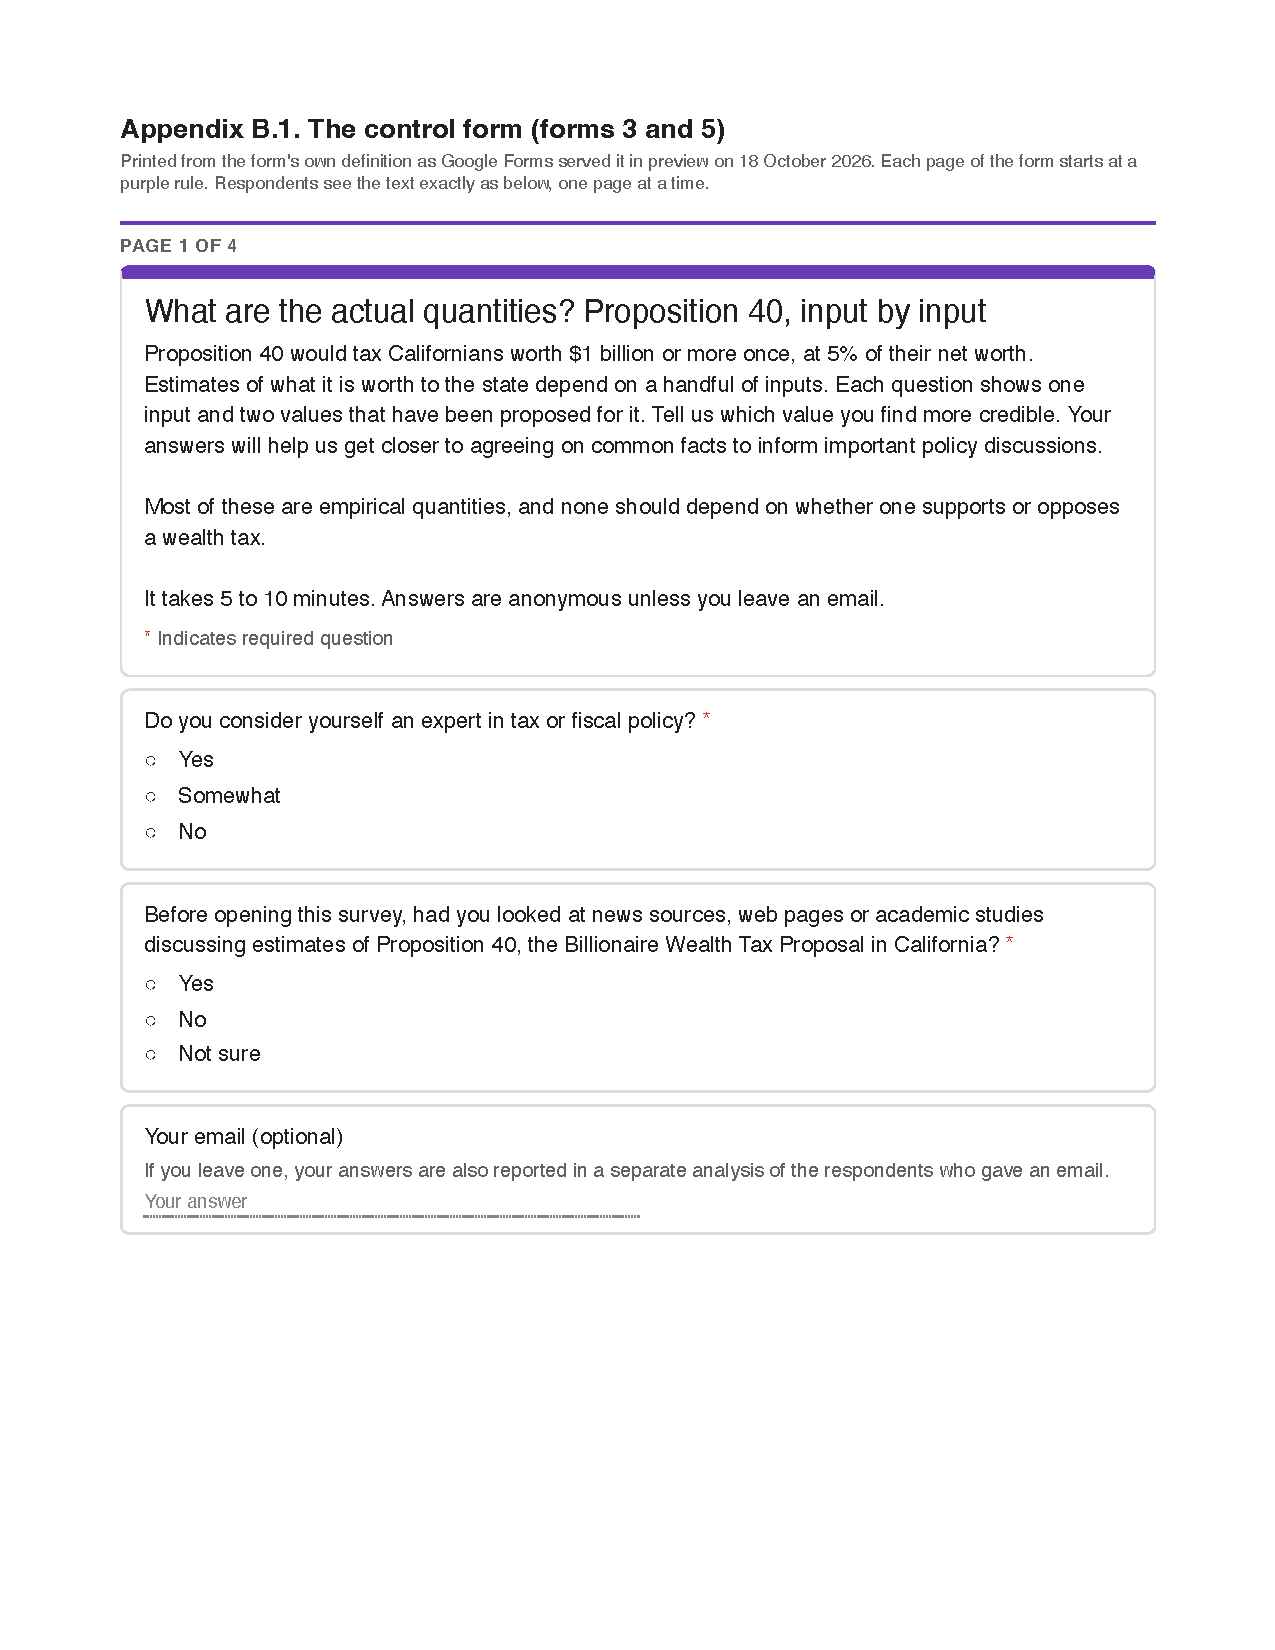
\includepdf[pages=-,pagecommand={\thispagestyle{plain}}]{forms/control.pdf}
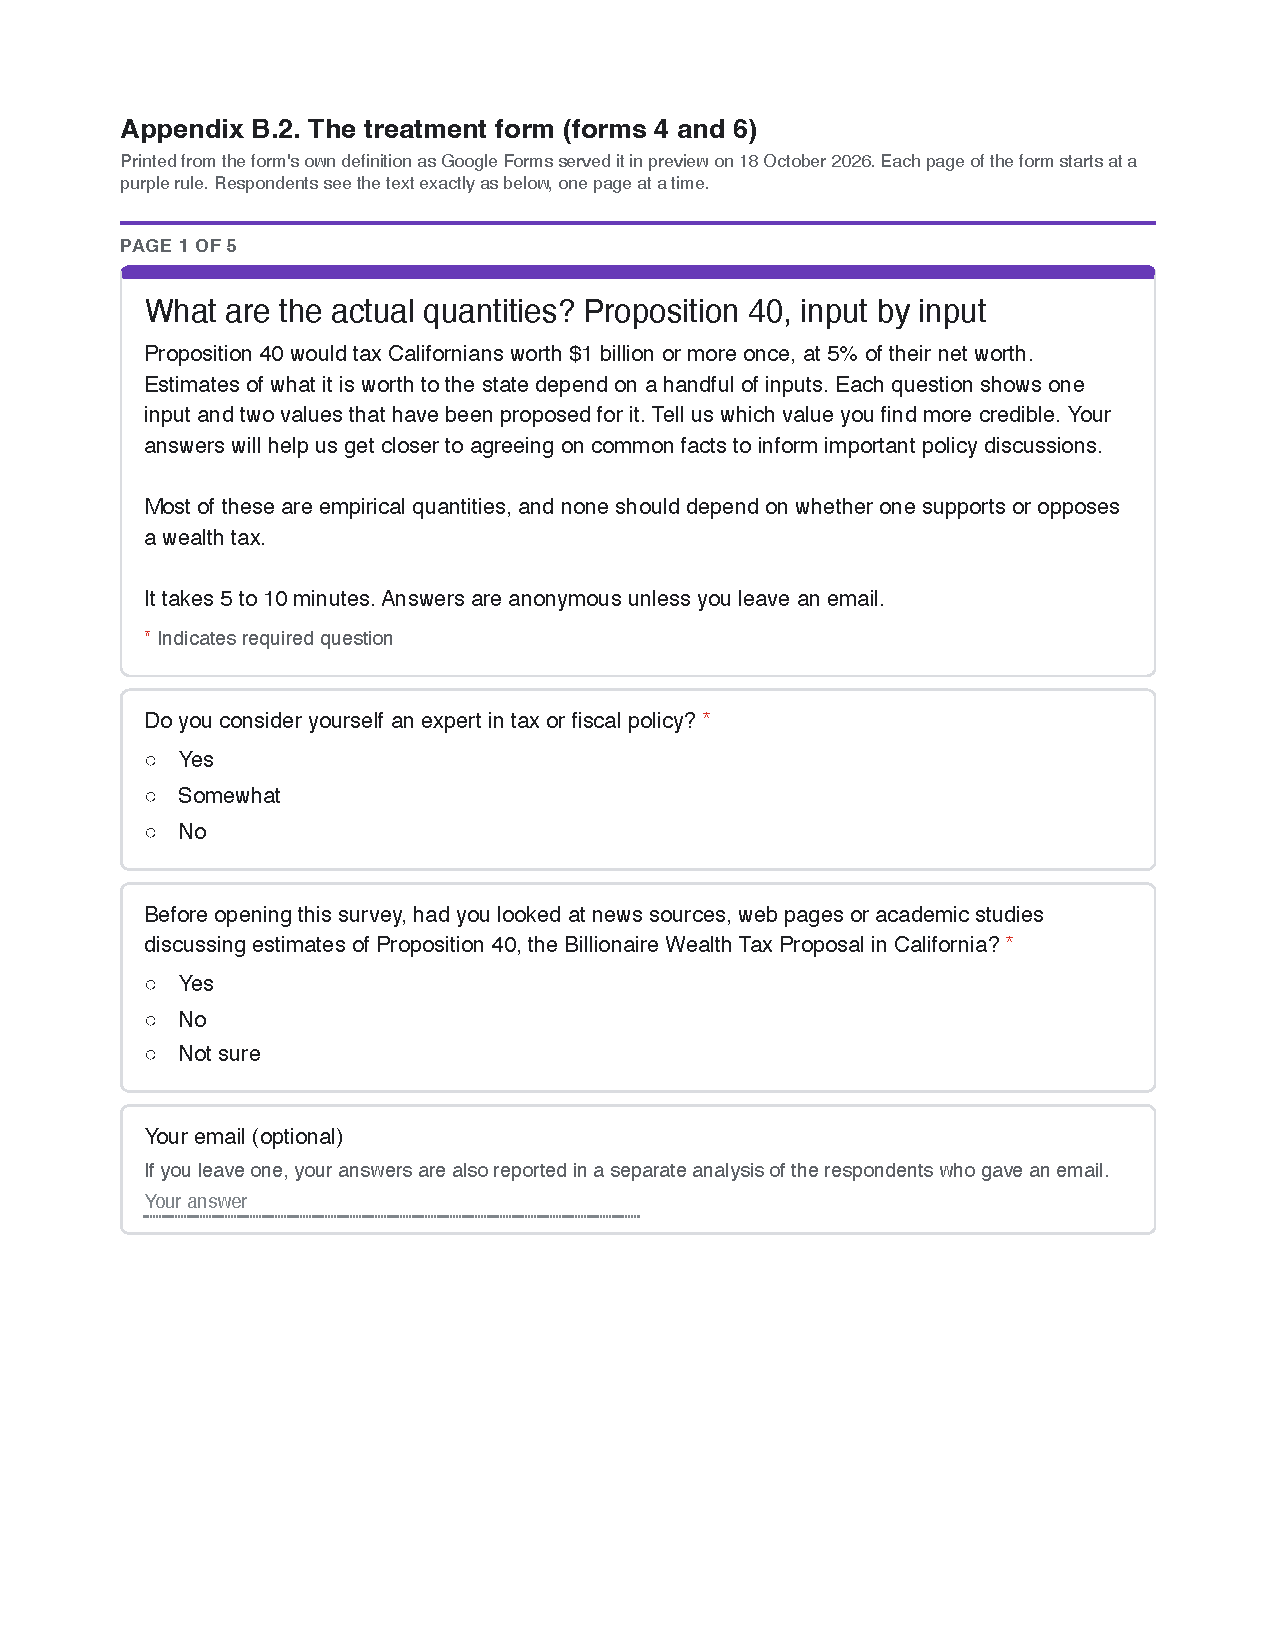
\includepdf[pages=-,pagecommand={\thispagestyle{plain}}]{forms/treatment.pdf}
\end{document}
